\section*{Encaminamiento por vector-distancia, direccionamiento IP y detecci\'on de errores con CRC}

\begin{enumerate}
    \item Aplique el algoritmo de encaminamiento de vector-distancia a la siguiente topolog\'ia de red.
    \begin{enumerate}
        \item Indique el estado de las tablas de ruteo para las etapas de cold-start y luego para el env\'io de los primeros dos mensajes.
        \item Luego, indique el estado de las tablas de ruteo para el estado estacionario.
        \item Una vez alcanzado el estado estacionario , el enlace 6 se rompe. Descria la manera en c\'omo procede el protocolo hasta retomar
        un nuevo estado estacionario.
        \item ¿Qu\'e fen\'omeno podr\'ia causar un bucle de ruteo?
        \item Finalmente, ¿cu\'al protocolo en la pr\'actica implementa el algoritmo de vector-distancia? ¿cu\'al es la frecuencia de los mensajes
        de refresco y cu\'al es la finalidad de los mismos?

        \begin{figure}[H]
            \centering
            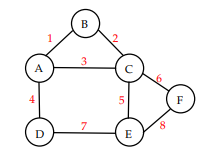
\includegraphics[width=0.35\textwidth]{img/Vector-distancia.png}
        \end{figure}
    \end{enumerate}

    \item Suponga que le han asignado el bloque de red 132.46.0.0/16 y que necesita configurar ocho subredes.
    \begin{enumerate}
        \item ¿Cu\'antos d\'igitos binarios se requieren para definir ocho subredes?
        \item Especifique el prefijo de red extendido que permite la creaci\'on de las 8 subredes.
        \item Exprese las direcciones de subred en formato binario y decimal.
        \item Enliste el rango de direcciones IP que pueden asignarse a la subred n\'umero 4.
        \item ¿Cu\'al es la direcci\'on de difusi\'on (\textit{broadcast}) de la subred n\'umero 4?
    \end{enumerate}

    \item Suponga que se le ha asignado el bloque de direcciones de red 200.30.1.0/24.
    \begin{enumerate}
        \item Defina un prefijo de red extendido que permita crear 20 estaciones en cada subred.
        \item 
    \end{enumerate}
\end{enumerate}